%% =============================================================================
%% main.tex -- IEEE conference paper skeleton (IEEEtran, two-column)
%% Project : PPG-based respiratory-rate estimation with conformal prediction
%%
%% HOW TO USE ON OVERLEAF
%%   1. Upload this folder (main.tex, references.bib, figures/) as a project.
%%   2. Menu -> Compiler = pdfLaTeX, Main document = main.tex.
%%   3. Search the source for "TODO" (red text in the PDF) and "PLACEHOLDER".
%%   4. Before submission: delete the \TODO / \figplaceholder helper macros,
%%      all red text, and every comment line that starts with "%%".
%%
%% COLOUR CODE IN THE PDF
%%   red   = something you must supply or verify (TODO / placeholder figure)
%%   black = draft text and numbers copied from your project results
%% =============================================================================
\documentclass[conference]{IEEEtran}
\IEEEoverridecommandlockouts
% The preceding line is only needed to identify funding in the first footnote.
% If that is unneeded, please comment it out.
\usepackage{cite}
\usepackage{amsmath,amssymb,amsfonts}
\usepackage{algorithmic}
\usepackage{graphicx}
\usepackage{textcomp}
\usepackage{xcolor}
\usepackage{booktabs}   % professional table rules (\toprule, \midrule, \bottomrule)
\usepackage{multirow}
\usepackage{array}
\usepackage{url}
\ifCLASSOPTIONcompsoc
 \usepackage[caption=false,font=normalsize,labelfont=sf,textfont=sf]{subfig}
\else
 \usepackage[caption=false,font=footnotesize]{subfig}
\fi
\def\BibTeX{{\rm B\kern-.05em{\sc i\kern-.025em b}\kern-.08em
    T\kern-.1667em\lower.7ex\hbox{E}\kern-.125emX}}

\graphicspath{{figures/}}

%% ---- helper macros (remove before submission) -------------------------------
\newcommand{\TODO}[1]{{\color{red}\textbf{[TODO: #1]}}}
\newcommand{\figplaceholder}[2]{%
  \fbox{\parbox[c][#1][c]{0.92\linewidth}{\centering\color{red}%
  \textbf{PLACEHOLDER FIGURE}\\[2pt]\footnotesize #2}}}

%% ---- notation macros ----------------------------------------------------------
\newcommand{\bpm}{bpm}
\newcommand{\Cset}{\mathcal{C}_{\alpha}}
\DeclareMathOperator{\SQI}{SQI}

\makeatletter
\newcommand{\linebreakand}{%
  \end{@IEEEauthorhalign}
  \hfill\mbox{}\par
  \mbox{}\hfill\begin{@IEEEauthorhalign}
}
\makeatother

\begin{document}

%% -----------------------------------------------------------------------------
%% TITLE  (no math, symbols, footnotes or sub-title in the title)
%% Alternatives you may prefer:
%%   - Conformal Prediction for Respiratory Rate Estimation from Photoplethysmography:
%%     Selective Triage and Behavior Under Domain Shift
%%   - Can We Trust PPG Respiratory Rate? A Patient-Disjoint Study of Conformal
%%     Intervals, Abstention, and External Validation
%% -----------------------------------------------------------------------------
\title{Uncertainty-Aware Respiratory Rate Estimation from Photoplethysmography: Conformal Prediction, Selective Triage, and Failure Under Domain Shift}
%\thanks{Identify applicable funding agency here. If none, delete this.}

\author{\IEEEauthorblockN{1\textsuperscript{st} Santhosh R}
\IEEEauthorblockA{\textit{SRM Institute of Science and Technology} \\
Kattankulathur, Chengalpattu, Tamil Nadu, India \\
santhosh7x17@gmail.com}
\and
\IEEEauthorblockN{2\textsuperscript{nd} Visshva R}
\IEEEauthorblockA{\textit{SRM Institute of Science and Technology} \\
Kattankulathur, Chengalpattu, Tamil Nadu, India \\
visshva.ramasubramanian@gmail.com}
\linebreakand
\IEEEauthorblockN{3\textsuperscript{rd} Joe Infant Arockiasamy}
\IEEEauthorblockA{\textit{SRM Institute of Science and Technology} \\
Kattankulathur, Chengalpattu, Tamil Nadu, India \\
ja7218@srmist.edu.in}
\and
\IEEEauthorblockN{4\textsuperscript{th} Joel Sheno G}
\IEEEauthorblockA{\textit{SRM Institute of Science and Technology} \\
Kattankulathur, Chengalpattu, Tamil Nadu, India \\
jg6993@srmist.edu.in}
\linebreakand
\IEEEauthorblockN{5\textsuperscript{th} Uma E\textsuperscript{*}}
\IEEEauthorblockA{\textit{Assistant Professor} \\
\textit{SRM Institute of Science and Technology} \\
Kattankulathur, Chengalpattu, Tamil Nadu, India \\
\textsuperscript{*}Corresponding author}
}

\maketitle

%% -----------------------------------------------------------------------------
%% ABSTRACT: 150--250 words. No math, symbols, citations or footnotes.
%% Every number below comes from your results files; re-check after you fix the
%% canonical evaluation protocol (see the consistency notes in the chat).
%% -----------------------------------------------------------------------------
\begin{abstract}
Respiratory rate is a key vital sign, and photoplethysmography from pulse oximeters offers a low-cost way to estimate it continuously, yet a point estimate gives no indication of when it can be trusted. We present a CPU-only pipeline that estimates respiratory rate from 60-second photoplethysmogram windows using 28 pulse-modulation features and gradient-boosted trees, wraps the predictions in split and cross-fitted conformal prediction intervals, and abstains using interval width combined with a signal quality index. Under strict patient-disjoint evaluation on 53 intensive care patients, the model reaches a mean absolute error of 1.81 breaths per minute versus 2.13 for a train-median baseline, and the patient-clustered bootstrap interval for the difference excludes zero. Nominal 90 percent intervals reach 87.4 percent mean coverage, but coverage across folds ranges from 68 to 100 percent, and cross-fitting does not remove this spread, which points to between-patient heterogeneity rather than small calibration sets. A logistic combination of interval width and signal quality reaches an area under the receiver operating characteristic curve of 0.75 for flagging large errors on clean windows, and retaining 60 percent of windows lowers the error to 1.18 breaths per minute. Zero-shot transfer to the CapnoBase benchmark gives an error of 3.80 breaths per minute for spontaneously breathing adults but 7.76 breaths per minute and 24 percent coverage for mechanically ventilated adults, showing that conformal validity breaks under physiological domain shift.
\end{abstract}

\begin{IEEEkeywords}
photoplethysmography, respiratory rate, conformal prediction, uncertainty quantification, selective prediction, domain shift, patient monitoring
\end{IEEEkeywords}

%% =============================================================================
\section{Introduction}\label{sec:intro}
Respiratory rate (RR) is among the earliest vital signs to deteriorate in acutely ill patients, yet it is still frequently recorded by manual counting. Pulse oximeters already provide a photoplethysmogram (PPG) at almost every bedside, and respiration modulates this waveform through changes in pulse amplitude, baseline, and pulse interval, which makes continuous PPG-based RR estimation attractive \cite{karlen2013,charlton2018review,pimentel2016}. Recent work improves point accuracy with handcrafted features and gradient boosting \cite{lee2022rr} or deep networks \cite{chin2024rr}, and wearable PPG is increasingly common \cite{kim2023ppg}.

A clinically useful monitor must also say when it should not be trusted. Motion, poor perfusion, and sensor displacement degrade the PPG \cite{zheng2024tinyppg,zhao2026sqi}, and patients differ widely in physiology. Distribution-free conformal prediction offers prediction intervals with a finite-sample marginal coverage guarantee under exchangeability \cite{vovk2005,lei2018distfree,angelopoulos2021gentle}, and a reject option lets a model abstain on uncertain inputs \cite{hendrickx2024reject}. Conformal methods have been applied to clinical time series and PPG classification \cite{dalal2025sepsis,kinalioglu2026conformal}, but we are not aware of a patient-disjoint benchmark for \emph{continuous} PPG respiratory-rate regression that examines interval validity, abstention, and external transfer together. \TODO{Verify this novelty statement with a targeted literature search before submission.}

Two properties of physiological data challenge the conformal guarantee. First, windows from one patient are strongly correlated (our 60-s windows overlap by 97\%), so the effective number of independent units is the number of patients, not windows. Second, a model trained on one clinical population may face a different physiology at deployment. We therefore evaluate with patient-disjoint folds and test on an independent external cohort.

\textbf{Contributions.}
\begin{itemize}
\item A leakage-free, patient-disjoint benchmark of PPG respiratory-rate estimation on 53 ICU patients with 28 physiologically grounded features, a trivial train-median baseline, and classical spectral and pulse-modulation baselines.
\item A comparison of five conformal configurations (including a train-median baseline) and CV+ cross-fitting, showing that fold-to-fold coverage instability persists across all of them.
\item An analysis of interval width, a signal quality index (SQI), and their combination for detecting corrupted windows and large errors, with risk--coverage curves bounded by oracle and random abstention.
\item A zero-shot external validation on CapnoBase stratified by age and ventilation mode, documenting where conformal validity fails.
\item A CPU-only, deterministic, open implementation \TODO{insert repository URL}.
\end{itemize}

The remainder of the paper is organized as follows. Section~\ref{sec:related} reviews related work, Section~\ref{sec:data} describes the data, Section~\ref{sec:method} presents the method, Section~\ref{sec:results} reports results, Section~\ref{sec:discussion} discusses findings and limitations, and Section~\ref{sec:conclusion} concludes.

%% =============================================================================
\section{Related Work}\label{sec:related}
\subsection{PPG-Based Respiratory Rate Estimation}
Respiration is commonly extracted from PPG as respiratory-induced amplitude, intensity, and frequency variations, which are fused or fed to learned models \cite{karlen2013,charlton2018review}. The BIDMC dataset was introduced as a benchmark for pulse-oximeter RR algorithms \cite{pimentel2016}. Lee et al.\ combine autocorrelation-based spectral features with gradient boosting and report a mean absolute error of 1.94 bpm on BIDMC using 32-s windows with 10-fold cross-validation \cite{lee2022rr}, and Chin et al.\ evaluate a CNN-LSTM on 32-s windows of CapnoBase and BIDMC \cite{chin2024rr}. These studies report point estimates under random window splitting rather than patient-disjoint folds; protocols differ from ours in window length and splitting, so numbers are not directly comparable.

\subsection{Signal Quality and Artifacts}
Signal quality assessment improves downstream estimation: filtering low-quality segments reduced heart-rate error substantially in clinical wrist PPG \cite{zhao2026sqi}, and lightweight networks detect motion artifacts on edge devices \cite{zheng2024tinyppg}. These works classify quality; they do not attach calibrated intervals to the downstream estimate.

\subsection{Conformal Prediction and Selective Prediction}
Split conformal prediction \cite{vovk2005,lei2018distfree}, conformalized quantile regression \cite{romano2019cqr}, and jackknife+/CV+ \cite{barber2021jackknife} give distribution-free intervals; extensions address covariate shift and non-exchangeable data \cite{tibshirani2019covshift,barber2023beyond}. Abstention has a long history \cite{chow1970reject,geifman2017selective} and is surveyed in \cite{hendrickx2024reject}.

\subsection{Conformal Prediction in Clinical and Physiological Settings}
Dalal et al.\ pair an RNN with conformal prediction for sepsis and report fewer false alarms \cite{dalal2025sepsis}. Kinalioglu audits conformal reliability of PPG-based ICU arrhythmia classification and shows that marginal coverage can hide failures on rare rhythms and individual patients \cite{kinalioglu2026conformal}. Shang applies split and sequential conformal prediction to functional time series of mortality rates \cite{shang2026conformal}. Table~\ref{tab:related} summarizes how these works relate to ours.

% >>> OPTIONAL: cut this table first if you run over the page limit
\begin{table}[!t]
\caption{Closest related work and the gap addressed here}
\label{tab:related}
\centering\footnotesize
\renewcommand{\arraystretch}{1.1}
\begin{tabular}{@{}p{0.85cm}p{3.55cm}p{3.1cm}@{}}
\toprule
\textbf{Ref.} & \textbf{Task and method} & \textbf{Gap here} \\
\midrule
\cite{lee2022rr} & RR from PPG; autocorrelation features, gradient boosting & Point estimate only \\
\cite{chin2024rr} & RR from PPG; CNN-LSTM & Point estimate; heavier training \\
\cite{zhao2026sqi} & Signal-quality classification before HR estimation & No prediction intervals \\
\cite{zheng2024tinyppg} & Edge motion-artifact detection & No uncertainty on the estimate \\
\cite{dalal2025sepsis} & RNN with conformal wrapper (sepsis, EHR) & Classification, not biosignal regression \\
\cite{kinalioglu2026conformal} & Conformal audit of PPG arrhythmia classification & Classification task \\
\cite{shang2026conformal} & Conformal intervals for functional time series & Demographic data \\
\textbf{Ours} & \textbf{RR regression, conformal intervals, abstention, external test} & \textbf{--} \\
\bottomrule
\end{tabular}
\end{table}

%% =============================================================================
\section{Data and Problem Formulation}\label{sec:data}
\subsection{Datasets}
\textbf{BIDMC} \cite{pimentel2016,goldberger2000}: 53 adult ICU patients, each with an 8-minute recording of fingertip PPG at 125 Hz and a synchronous reference respiratory signal from impedance pneumography. We cut each recording into 60-s windows with a 2-s stride, giving 11\,026 windows (54 to 211 per patient, mean 208). One patient (bidmc13) has a disconnected reference sensor for large parts of the record (30.4\% missing and 47.8\% near zero); we retain it to avoid post-hoc exclusion.

\textbf{CapnoBase} \cite{karlen2013}: an independent benchmark of 42 surgical cases (13 adults, 29 children; 23 breathing spontaneously, 19 mechanically ventilated), used \emph{only} for zero-shot testing with models frozen on BIDMC. Table~\ref{tab:cohorts} summarizes both cohorts.

\begin{table}[!t]
\caption{Cohorts used in this study}
\label{tab:cohorts}
\centering\footnotesize
\renewcommand{\arraystretch}{1.1}
\begin{tabular}{@{}p{1.9cm}p{2.7cm}p{3.3cm}@{}}
\toprule
 & \textbf{BIDMC} & \textbf{CapnoBase} \\
\midrule
Patients & 53 adult ICU & 42 surgical (13 adult, 29 pediatric) \\
Breathing mode & Spontaneous (adult ICU) & 23 spontaneous, 19 ventilated \\
PPG sampling & 125 Hz & 300 Hz (resampled to 125 Hz) \\
Reference RR & Impedance pneumography & Capnography ($Et\text{CO}_2$ annotations) \\
60-s windows & 11\,026 & 8\,764 \\
Role & Train, validate, calibrate, test & Zero-shot test only \\
\bottomrule
\end{tabular}
\end{table}

\subsection{Problem Formulation}
For window $i$ with feature vector $\mathbf{x}_i\in\mathbb{R}^{28}$ and reference respiratory rate $y_i$ (breaths per minute, bpm), we seek a point estimate $\hat{y}_i$ and an interval $\Cset(\mathbf{x}_i)$ with nominal coverage $1-\alpha=0.90$, together with an abstention rule that withholds unreliable estimates.

%% =============================================================================
\section{Methodology}\label{sec:method}
Fig.~\ref{fig:pipeline} gives an overview of the pipeline.

\begin{figure*}[!t]
\centering
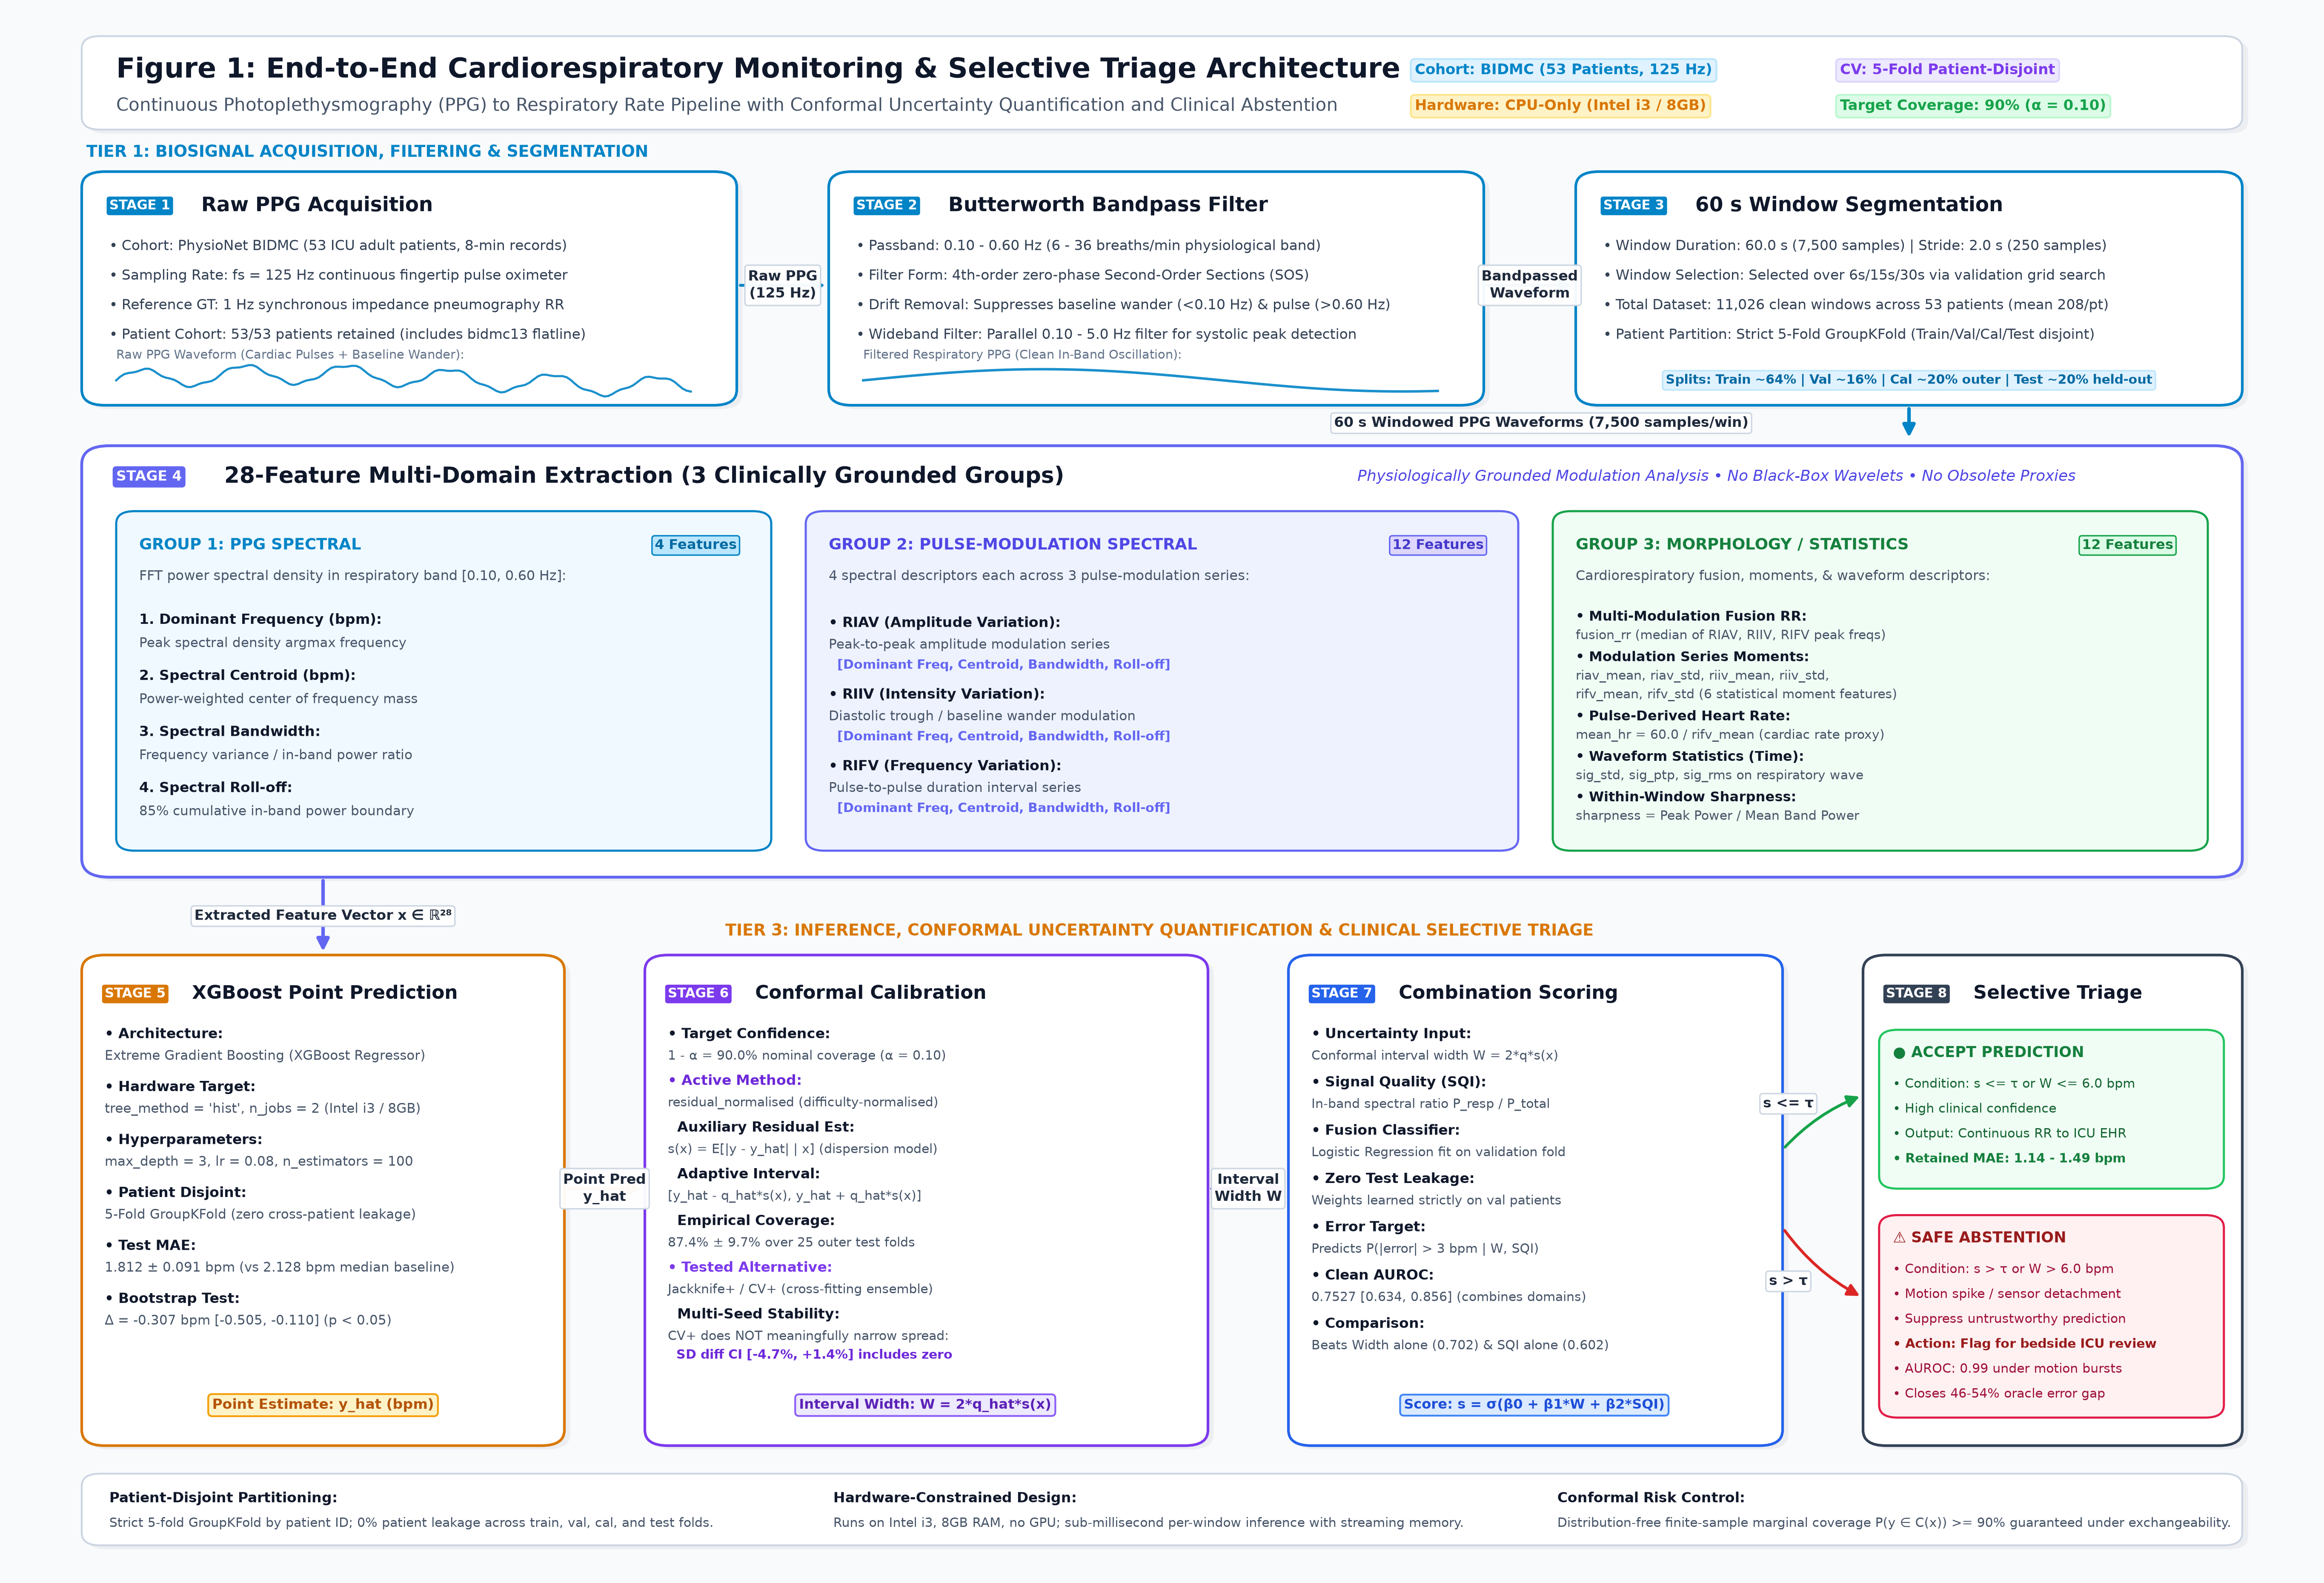
\includegraphics[width=0.95\textwidth]{pipeline_architecture.png}
\caption{Overview of the pipeline: bandpass filtering, 60-s windowing, 28-feature extraction, gradient-boosted regression, conformal calibration, combination scoring, and selective triage.}
\label{fig:pipeline}
\end{figure*}

\subsection{Preprocessing and Windowing}
PPG is filtered with a 4th-order zero-phase Butterworth bandpass (second-order sections) over 0.10--0.60 Hz (6--36 bpm) for the respiratory band, and in parallel over 0.10--5.0 Hz for pulse detection. Windows are 60 s with a 2-s stride; the window length was selected on validation patients from $\{6, 15, 30, 60\}$ s.

\subsection{Pulse-Modulation Features}
We extract three respiratory-induced series: amplitude variation (RIAV), intensity variation (RIIV), and frequency variation (RIFV). From each 60-s window we compute 28 features in four groups (Table~\ref{tab:features}).

\begin{table}[!t]
\caption{Feature groups (28 features in total)}
\label{tab:features}
\centering\footnotesize
\renewcommand{\arraystretch}{1.1}
\begin{tabular}{@{}p{2.55cm}cp{4.2cm}@{}}
\toprule
\textbf{Group} & \textbf{\#} & \textbf{Descriptors} \\
\midrule
PPG spectral & 4 & Dominant frequency, centroid, bandwidth, roll-off in the 0.10--0.60 Hz band \\
Modulation spectral & 12 & Same four descriptors for each of RIAV, RIIV, RIFV \\
Modulation statistics & 8 & Fusion RR (median of the three modulation estimates), mean and SD of each series, mean heart rate \\
Morphology and sharpness & 4 & Window SD, peak-to-peak, RMS, spectral-peak sharpness \\
\bottomrule
\end{tabular}
\end{table}

\subsection{Point Regression}
A histogram-based XGBoost regressor \cite{chen2016xgboost} predicts $\hat{y}=f_\theta(\mathbf{x})$ (max depth 3, learning rate 0.08, 100 trees, subsample 0.85, column sample 0.80; $L_1$/$L_2$ regularization 0.5/2.0), with hyperparameters chosen on validation patients only. Seeds and thread counts are fixed so runs are bit-identical.

\subsection{Difficulty-Normalized Split Conformal Prediction}
An auxiliary regressor $\hat{\sigma}(\mathbf{x})$ is trained on grouped out-of-fold absolute residuals to estimate difficulty. On the calibration patients we compute normalized scores
\begin{equation}
s_i=\frac{|y_i-\hat{y}_i|}{\hat{\sigma}(\mathbf{x}_i)},\qquad i\in\mathcal{D}_{\mathrm{cal}},\label{eq:score}
\end{equation}
and take the conformal quantile
\begin{equation}
\hat{q}=\text{the } \lceil (n+1)(1-\alpha)\rceil\text{-th smallest of } \{s_i\}_{i=1}^{n},\label{eq:qhat}
\end{equation}
where $n$ is the number of calibration windows. The interval and its width are
\begin{equation}
\Cset(\mathbf{x})=\big[\hat{y}-\hat{q}\,\hat{\sigma}(\mathbf{x}),\ \hat{y}+\hat{q}\,\hat{\sigma}(\mathbf{x})\big],\quad W(\mathbf{x})=2\hat{q}\,\hat{\sigma}(\mathbf{x}).\label{eq:interval}
\end{equation}
Under exchangeability, $\Pr[y\in\Cset(\mathbf{x})]\ge 1-\alpha$ marginally \cite{vovk2005,lei2018distfree}. Because windows within a patient are correlated, this assumption holds at best across patients, which we test empirically. We compare it with three alternative scores on the same XGBoost predictions (absolute residual, Mondrian terciles, spectral sharpness), with a train-median baseline, and with CV+.

\textbf{CV+.} We also evaluate jackknife+/CV+ \cite{barber2021jackknife} with patient-grouped inner folds. With $k(i)$ the inner fold of window $i$, $\hat{\mu}_{-k(i)}$ the model fitted without that fold, and $R_i=|y_i-\hat{\mu}_{-k(i)}(\mathbf{x}_i)|$,
\begin{equation}
\Cset^{\mathrm{CV+}}(\mathbf{x})=\Big[\hat{q}^{-}_{\alpha}\{\hat{\mu}_{-k(i)}(\mathbf{x})-R_i\},\ \hat{q}^{+}_{\alpha}\{\hat{\mu}_{-k(i)}(\mathbf{x})+R_i\}\Big],\label{eq:cvplus}
\end{equation}
where $\hat{q}^{-}_{\alpha}$ and $\hat{q}^{+}_{\alpha}$ are the lower and upper $\alpha$ empirical quantiles.

\subsection{Signal Quality, Combination Score, and Selective Triage}
The SQI abstention score is one minus the fraction of window power inside the respiratory band, so higher means worse quality. A logistic regression fitted on validation patients combines width and SQI into
\begin{equation}
\begin{split}
g(\mathbf{x})&=\sigma\big(\beta_0+\beta_1 W(\mathbf{x})+\beta_2\,\SQI(\mathbf{x})\big)\\
&\approx\Pr\big(|y-\hat{y}|>3\ \text{bpm}\mid\mathbf{x}\big),
\end{split}\label{eq:combo}
\end{equation}
with $\sigma$ the logistic function. A window is retained when $g(\mathbf{x})\le\tau$. The selective risk and retention are
\begin{equation}
R(\tau)=\mathbb{E}\big[|y-\hat{y}|\ \big|\ g(\mathbf{x})\le\tau\big],\qquad \phi(\tau)=\Pr[g(\mathbf{x})\le\tau],\label{eq:risk}
\end{equation}
and we plot $R$ against $\phi$ with oracle (abstain on the largest true errors) and random abstention as bounds.

\subsection{Raw-Signal Corruption}
To test artifact sensitivity we corrupt validation and test windows in the time domain \emph{before} feature extraction, leaving training and calibration data clean. Four composable artifacts (high-frequency noise, baseline drift, motion bursts, flatline dropouts) are applied at three severities, with achieved SNR of $+5.0\pm2.1$ dB (mild), $-5.5\pm3.8$ dB (moderate), and $-12.6\pm7.4$ dB (severe).

\subsection{Evaluation Protocol and Metrics}
Patients are split into disjoint train, validation, calibration, and test sets in five folds (8--9 calibration patients per fold), repeated with five fold-map seeds (42, 101, 202, 303, 404), giving 25 evaluations. We report mean absolute error (MAE), empirical coverage, mean interval width, the fold-level coverage range, patient-level coverage, and the AUROC for flagging $|{\rm error}|>3$ bpm. Confidence intervals use 1\,000 patient-clustered bootstrap resamples. Baselines are the train median and the classical spectral, RIAV, RIIV, RIFV, and fusion estimators.

%% =============================================================================
\section{Experimental Results}\label{sec:results}
\subsection{Point Accuracy}
Across the 25 repeated evaluations XGBoost reaches an MAE of $1.81\pm0.09$ bpm against $2.13\pm0.03$ bpm for the train median; the paired patient-clustered bootstrap difference is $-0.31$ bpm (95\% CI $[-0.51,-0.11]$). Table~\ref{tab:accuracy} places this against the classical estimators, none of which beats a constant prediction, and shows that the explained variance is modest ($R^2=0.09$). The within-patient MAE of a constant predictor (removing patient-specific mean bias) is only 0.63 bpm, which confirms that most of the residual error is between-patient variance, as illustrated in the prediction scatter plot (Fig.~\ref{fig:scatter_a}).

\begin{table}[!t]
\caption{Point accuracy under patient-disjoint 5-fold evaluation (one fold map, 60-s windows)}
\label{tab:accuracy}
\centering\footnotesize
\renewcommand{\arraystretch}{1.1}
\begin{tabular}{@{}lccc@{}}
\toprule
\textbf{Method} & \textbf{MAE (bpm)} & $\boldsymbol{R^2}$ & \textbf{Pearson} $\boldsymbol{r}$ \\
\midrule
Train median & $2.12\pm0.33$ & $-0.04$ & -- \\
Classical spectral & $2.54\pm0.67$ & $-1.58$ & 0.42 \\
RIAV & $3.95\pm1.00$ & $-4.19$ & 0.11 \\
RIIV & $2.95\pm0.95$ & $-2.48$ & 0.34 \\
RIFV & $5.82\pm0.53$ & $-7.49$ & 0.13 \\
Fusion (median) & $3.08\pm0.65$ & $-2.71$ & 0.28 \\
\textbf{XGBoost (28 features)} & $\mathbf{1.81}\pm0.42$ & $\mathbf{0.09}$ & 0.41 \\
\bottomrule
\end{tabular}
\par\vspace{2pt}{\footnotesize Mean $\pm$ SD across 5 cross-validation folds (sample SD, $\text{ddof}=1$).\par}
\end{table}

\subsection{Conformal Validity}
Table~\ref{tab:scores} compares five conformal configurations and CV+ at a 90\% target. Mean coverage is 84.5--87.5\% for split variants and 90.7\% for CV+, but no variant stabilizes coverage across folds: the min--max range is 29.7--38.0 percentage points for all methods, and CV+ is not significantly narrower than the difficulty-normalized score (bootstrap CI of the SD difference $[-4.7,+1.4]$ points, which includes zero). Table~\ref{tab:perfold} shows the calibration quantile $\hat{q}$ varying from 1.65 to 4.59 across folds, and Fig.~\ref{fig:foldcov} visualizes the fold-level spread. Because CV+ pools residuals from roughly five times more patients yet leaves the spread unchanged, the instability reflects between-patient heterogeneity rather than only the small calibration set. Patient-level coverage is similarly dispersed ($86.3\pm20.5\%$).

\begin{table*}[!t]
\caption{Conformal methods at 90\% nominal coverage, 25 folds (5 seeds $\times$ 5 folds). XGB is XGBoost. Error AUROC flags $|{\rm error}|>3$ bpm on clean windows; $\pm$ is the SD over folds.}
\label{tab:scores}
\centering\footnotesize
\renewcommand{\arraystretch}{1.1}
\setlength{\tabcolsep}{3pt}
\begin{tabular}{@{}lcccccc@{}}
\toprule
\textbf{Method} & \textbf{MAE (bpm)} & \textbf{Mean cov.\ (\%)} & \textbf{Cov.\ range (\%)} & \textbf{Width (bpm)} & \textbf{Error AUROC} & \textbf{Patient cov.\ (\%)} \\
\midrule
Train median & $2.13\pm0.41$ & $86.6\pm10.4$ & 67.3--100.0 & $9.59\pm2.84$ & 0.50 (const.) & $85.3\pm26.0$ \\
XGB, abs.\ residual & $1.81\pm0.43$ & $87.5\pm9.8$ & 65.5--100.0 & $8.54\pm2.86$ & 0.50 (const.) & $86.3\pm22.6$ \\
XGB, difficulty-normalized & $1.81\pm0.43$ & $87.4\pm9.7$ & 68.2--100.0 & $9.30\pm4.87$ & $0.68\pm0.12$ & $86.3\pm20.5$ \\
XGB, Mondrian terciles & $1.81\pm0.43$ & $84.5\pm10.3$ & 62.0--100.0 & $7.71\pm2.56$ & $0.52\pm0.12$ & $83.3\pm23.7$ \\
XGB, spectral sharpness & $1.81\pm0.43$ & $87.4\pm10.5$ & 64.5--100.0 & $8.64\pm3.16$ & $0.60\pm0.08$ & $86.2\pm22.8$ \\
Jackknife+ / CV+ & $1.73\pm0.38$ & $90.7\pm7.9$ & 70.2--100.0 & $8.98\pm1.16$ & $0.57\pm0.16$ & $89.4\pm20.6$ \\
\bottomrule
\end{tabular}
\end{table*}

% >>> OPTIONAL (supports the heterogeneity argument; cut if space is short)
\begin{table}[!t]
\caption{Per-fold calibration audit (seed 42)}
\label{tab:perfold}
\centering\footnotesize
\renewcommand{\arraystretch}{1.1}
\begin{tabular}{@{}cccccc@{}}
\toprule
\textbf{Fold} & $\boldsymbol{\hat{q}}$ & \textbf{Cal.\ pts.} & \textbf{MAE} & \textbf{Cov.\ (\%)} & \textbf{Width} \\
\midrule
0 & 1.65 & 8 & 2.18 & 76.2 & 5.88 \\
1 & 1.68 & 8 & 2.31 & 86.1 & 9.01 \\
2 & 2.10 & 8 & 2.02 & 74.1 & 5.81 \\
3 & 4.59 & 9 & 1.06 & 100.0 & 18.29 \\
4 & 3.66 & 9 & 1.33 & 95.3 & 16.18 \\
\bottomrule
\end{tabular}
\end{table}

\begin{figure}[!t]
\centering
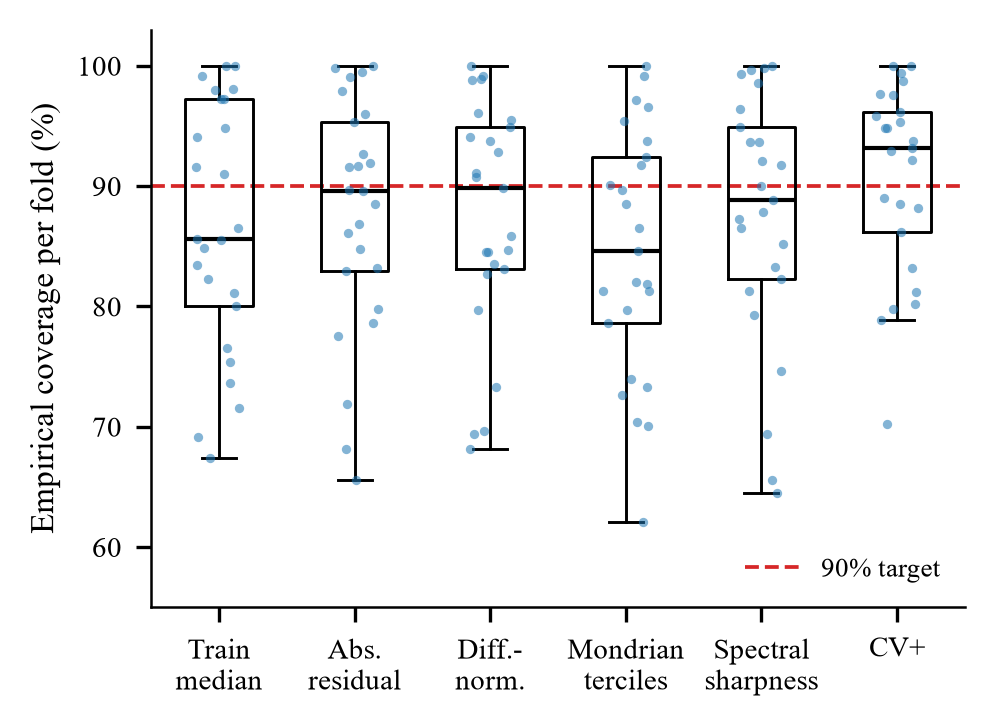
\includegraphics[width=0.9\linewidth]{fig2_fold_coverage.png}
\caption{Fold-level empirical coverage for each conformal method against the 90\% target.}
\label{fig:foldcov}
\end{figure}

\subsection{Detecting Corrupted Windows and Large Errors}
Table~\ref{tab:corrupt} shows that the SQI is a far better corruption detector than conformal width (AUROC 0.90, 0.99, and 1.00 for mild, moderate, and severe corruption versus 0.63--0.73 for raw width). On \emph{clean} windows the picture changes (Table~\ref{tab:clean}): raw width and SQI are statistically indistinguishable (0.61 versus 0.60, overlapping intervals), and their logistic combination has the highest point estimate (0.75, 95\% CI $[0.63,0.86]$), though confidence intervals overlap with the individual predictors. Fold-normalizing the width raises the pooled AUROC from 0.61 to 0.70 but leaves the per-fold AUROC unchanged ($0.68\pm0.15$ for both), because $\hat{q}$ is constant within a fold; the gain therefore reflects rescaling across folds, not a better ranking.

% >>> OPTIONAL: merge Tables corrupt and clean into one if space is short
\begin{table}[!t]
\caption{AUROC for separating corrupted from clean windows (95\% CI in brackets)}
\label{tab:corrupt}
\centering\footnotesize
\renewcommand{\arraystretch}{1.1}
\begin{tabular}{@{}lcc@{}}
\toprule
\textbf{Severity (SNR)} & \textbf{Raw width} & \textbf{SQI} \\
\midrule
Mild ($+5.0$ dB) & 0.63 [0.57, 0.69] & \textbf{0.90} [0.88, 0.92] \\
Moderate ($-5.5$ dB) & 0.67 [0.59, 0.74] & \textbf{0.99} [0.99, 1.00] \\
Severe ($-12.6$ dB) & 0.73 [0.65, 0.81] & \textbf{1.00} [1.00, 1.00] \\
\bottomrule
\end{tabular}
\end{table}

\begin{table}[!t]
\caption{AUROC for flagging $|{\rm error}|>3$ bpm on clean windows}
\label{tab:clean}
\centering\footnotesize
\renewcommand{\arraystretch}{1.1}
\begin{tabular}{@{}lcc@{}}
\toprule
\textbf{Predictor} & \textbf{Pooled [95\% CI]} & \textbf{Per-fold} \\
\midrule
Raw interval width & 0.61 [0.50, 0.72] & $0.68\pm0.15$ \\
Fold-normalized width & 0.70 [0.60, 0.80] & $0.68\pm0.15$ \\
SQI & 0.60 [0.51, 0.70] & $0.63\pm0.14$ \\
\textbf{Width + SQI (logistic)} & \textbf{0.75} [0.63, 0.86] & $0.71\pm0.11$ \\
\bottomrule
\end{tabular}
\end{table}

\subsection{Selective Triage}
Table~\ref{tab:risk} and Fig.~\ref{fig:risk} show that abstention reduces error on clean windows. Retaining 60\% of windows with the combination score lowers the MAE to 1.18 bpm, 34\% below random abstention (1.78 bpm), against an oracle bound of 0.54 bpm. At 40\% retention fold-normalized width alone is best (1.01 versus 1.14 bpm), while the combination is better from 50\% to 95\% retention (with 95\% bootstrap confidence bands shown in Fig.~\ref{fig:risk}).

\begin{table}[!t]
\caption{Selective triage MAE (bpm) on clean windows by retention}
\label{tab:risk}
\centering\footnotesize
\renewcommand{\arraystretch}{1.1}
\setlength{\tabcolsep}{4pt}
\begin{tabular}{@{}cccccc@{}}
\toprule
\textbf{Ret.} & \textbf{Raw} & \textbf{Norm.} & \textbf{Comb.} & \textbf{Oracle} & \textbf{Random} \\
 & \textbf{width} & \textbf{width} & \textbf{score} & & \\
\midrule
40\% & 1.20 & \textbf{1.01} & 1.14 & 0.33 & 1.82 \\
50\% & 1.59 & 1.26 & \textbf{1.15} & 0.43 & 1.82 \\
60\% & 1.71 & 1.41 & \textbf{1.18} & 0.54 & 1.78 \\
80\% & 1.83 & 1.64 & \textbf{1.41} & 0.87 & 1.79 \\
90\% & 1.85 & 1.67 & \textbf{1.57} & 1.19 & 1.79 \\
100\% & 1.80 & 1.80 & 1.80 & 1.80 & 1.80 \\
\bottomrule
\end{tabular}
\end{table}

\begin{figure}[!t]
\centering
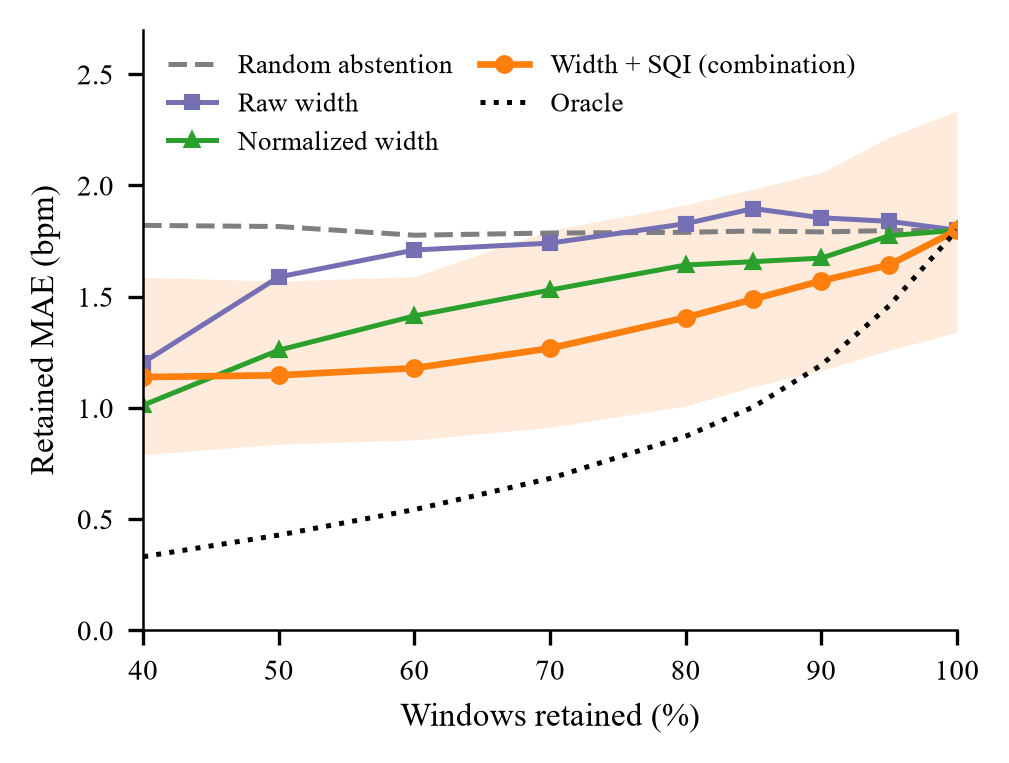
\includegraphics[width=0.9\linewidth]{fig3_risk_coverage.png}
\caption{Selective prediction on clean windows: retained MAE versus retention.}
\label{fig:risk}
\end{figure}

\begin{figure}[!t]
\centering
\subfloat[Predicted vs.\ reference respiratory rate.\label{fig:scatter_a}]{%
  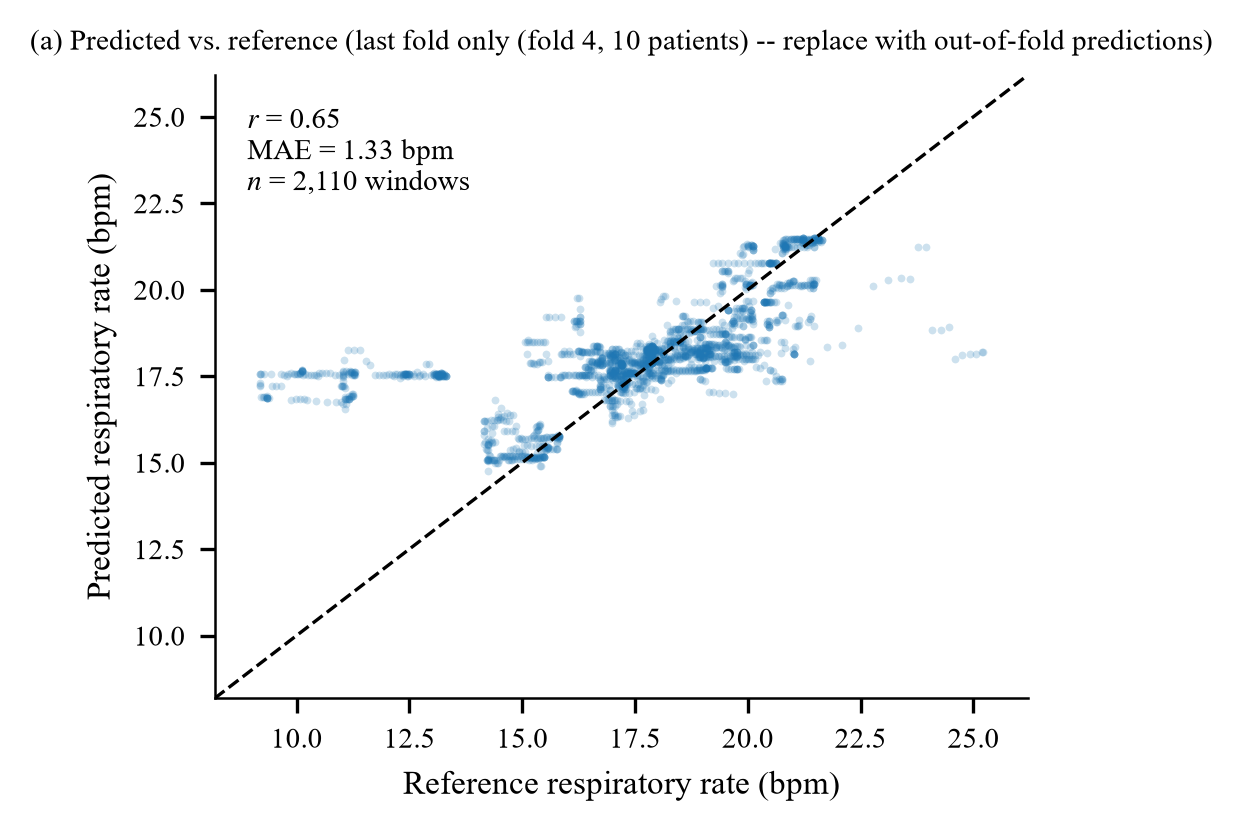
\includegraphics[width=0.92\linewidth]{fig4a_pred_vs_ref.png}%
}
\\[4pt]
\subfloat[Reference respiratory-rate distribution per cohort.\label{fig:scatter_b}]{%
  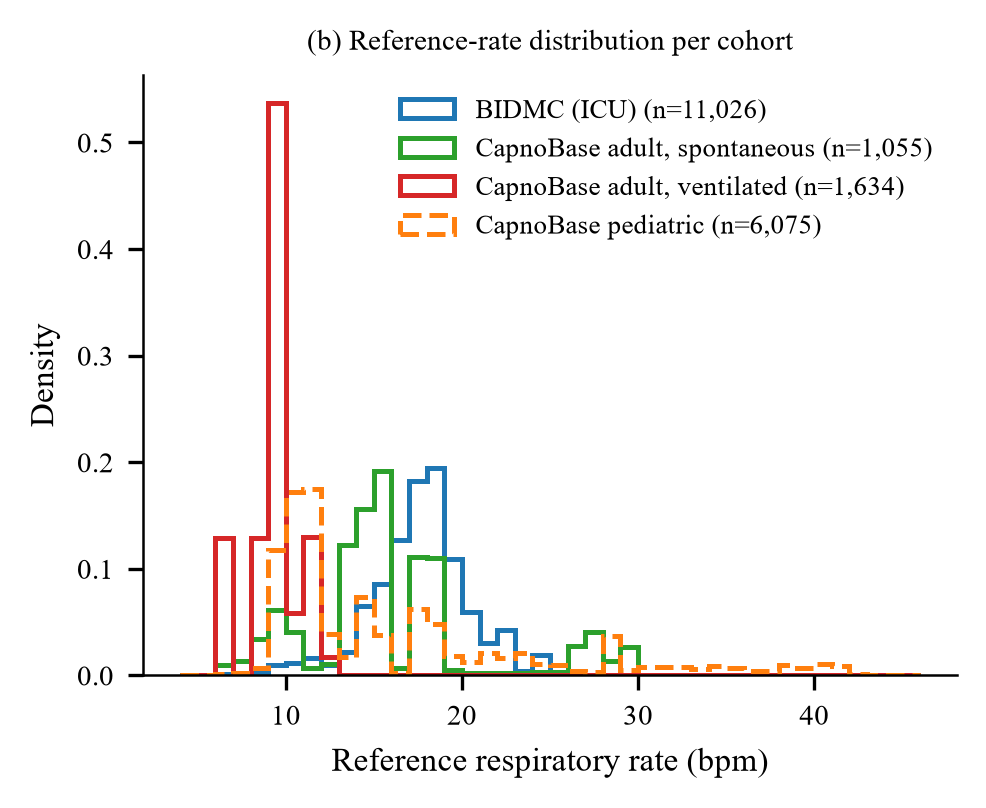
\includegraphics[width=0.92\linewidth]{fig4b_cohort_dist.png}%
}
\caption{Model predictions and cohort distributions: (a) predicted versus reference respiratory rate under patient-disjoint evaluation; (b) reference respiratory-rate distribution per cohort.}
\label{fig:scatter}
\end{figure}

\subsection{External Validation on CapnoBase}
Table~\ref{tab:external} and Fig.~\ref{fig:external} report zero-shot results with the five frozen BIDMC fold models and calibrators. Pediatric cases are partly outside the filter passband (4.5\% of windows above 36 bpm), so adults are the primary test. Within adults, ventilation mode separates the outcomes: spontaneously breathing adults ($N=5$) reach an MAE of 3.80 bpm with 77.7\% coverage, whereas mechanically ventilated adults ($N=8$) reach 7.76 bpm with 24.3\% coverage. Intervals widen only slightly (10.7 bpm in-domain versus 11.8--15.3 bpm outside), so the interval width does not warn of the failure, and the clean-window error AUROC falls to 0.45--0.62. Selective triage at 80\% retention still reduces the error (for example 3.48 bpm for spontaneous adults).

\begin{table*}[!t]
\caption{Zero-shot external validation (mean $\pm$ SD over the five BIDMC fold models)}
\label{tab:external}
\centering\footnotesize
\renewcommand{\arraystretch}{1.1}
\begin{tabular}{@{}lcccccc@{}}
\toprule
\textbf{Metric} & \textbf{BIDMC} & \textbf{Adult spont.} & \textbf{Adult vent.} & \textbf{Adult all} & \textbf{Pediatric} & \textbf{All 42} \\
 & ($N{=}53$) & ($N{=}5$) & ($N{=}8$) & ($N{=}13$) & ($N{=}29$) & \\
\midrule
MAE (bpm) & $1.78\pm0.55$ & $3.80\pm0.71$ & $7.76\pm0.40$ & $6.21\pm0.36$ & $6.39\pm0.29$ & $6.33\pm0.31$ \\
Coverage, 90\% target (\%) & $88.1\pm11.9$ & $77.7\pm14.6$ & $24.3\pm22.5$ & $45.3\pm18.4$ & $59.8\pm21.6$ & $55.3\pm20.3$ \\
Mean width (bpm) & $10.72\pm4.87$ & $12.16\pm6.32$ & $11.80\pm4.83$ & $11.94\pm5.39$ & $15.32\pm6.86$ & $14.29\pm6.32$ \\
Patient-level coverage (\%)$^{\mathrm{a}}$ & $87.1\pm19.2$ & $77.7\pm24.7$ & $23.7\pm21.3$ & $44.5\pm37.9$ & $59.8\pm37.4$ & $55.1\pm38.5$ \\
Error AUROC ($|{\rm err}|>3$) & $0.71\pm0.13$ & $0.54\pm0.12$ & $0.45\pm0.12$ & $0.53\pm0.15$ & $0.62\pm0.10$ & $0.58\pm0.10$ \\
Triage MAE, 80\% retention (bpm) & -- & $3.48\pm0.72$ & $7.86\pm0.39$ & $6.17\pm0.44$ & $5.97\pm0.35$ & $5.98\pm0.31$ \\
\textbf{Train-median MAE (bpm)} & $2.12\pm0.36$ & $4.07\pm0.09$ & $7.70\pm0.23$ & $6.28\pm0.17$ & $6.77\pm0.07$ & $6.62\pm0.10$ \\
\bottomrule
\multicolumn{7}{@{}l}{\footnotesize $^{\mathrm{a}}$ $\pm$ is the spread across patients within a fold, averaged over folds; other rows use the SD across folds.}
\end{tabular}
\end{table*}

\begin{figure*}[!t]
\centering
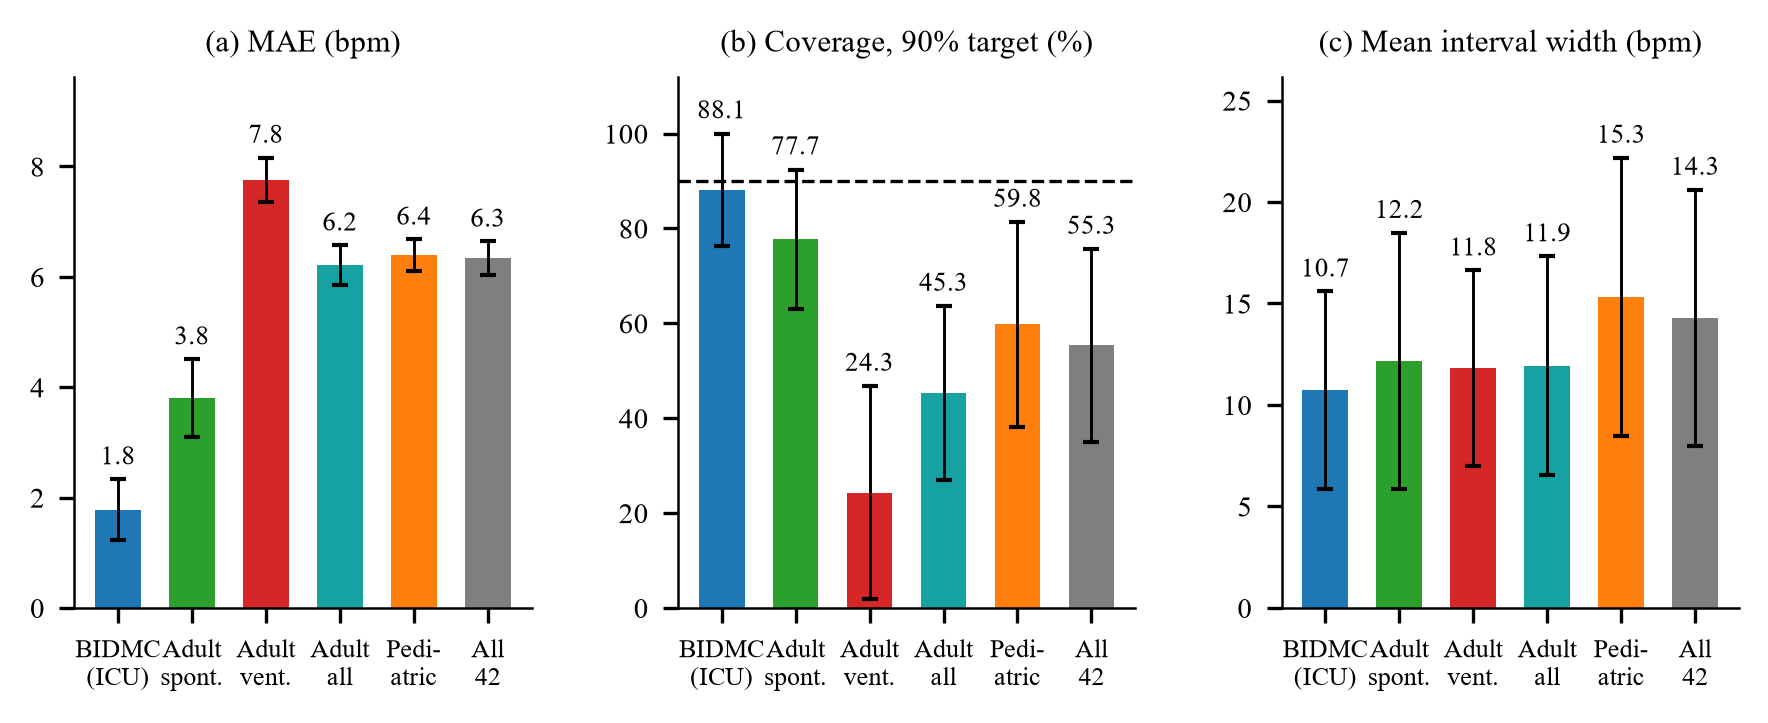
\includegraphics[width=0.95\textwidth]{fig5_external_validation.png}
\caption{External validation on CapnoBase: (a) MAE, (b) empirical coverage against the 90\% target, and (c) mean interval width across cohorts.}
\label{fig:external}
\end{figure*}

%% =============================================================================
\section{Discussion}\label{sec:discussion}
\subsection{Findings}
First, PPG respiratory-rate estimation on BIDMC under patient-disjoint evaluation improves only modestly on a constant predictor (1.81 versus 2.13 bpm); the value of the model lies as much in its uncertainty as in its point accuracy. Second, conformal intervals reach roughly nominal \emph{mean} coverage, but coverage varies from 62\% to 100\% across folds and from patient to patient, and neither alternative scores nor cross-fitting remove this; a marginal guarantee should not be read as a per-patient one, consistent with audits of PPG-based classifiers \cite{kinalioglu2026conformal}. Third, SQI and conformal width carry complementary information: SQI detects gross corruption almost perfectly, while width adds information about errors on clean windows. Fourth, conformal validity fails under a physiological domain shift, and the interval width does not signal it.

\subsection{Why Ventilated Patients Fail}
The 24\% coverage in ventilated adults is the clearest breach of exchangeability. A plausible explanation is that positive-pressure ventilation reverses the intrathoracic pressure cycle and changes how respiration modulates the pulse waveform. An alternative explanation is label shift: controlled ventilator rates differ from the ICU training distribution, and a model that leans on the training prior will err regardless of waveform physiology. Indeed, the train-median baseline yields an MAE of $7.70\pm0.23$ bpm on ventilated adults, essentially matching the $7.76\pm0.40$ bpm of XGBoost (Table~\ref{tab:external}), and the cohort reference-rate distributions (Fig.~\ref{fig:scatter_b}) reveal a distinct unimodal spike around typical ventilator settings ($\approx 12$ bpm). This supports the hypothesis that label shift contributes substantially alongside altered cardiopulmonary hemodynamics. Methods for covariate shift and non-exchangeable data \cite{tibshirani2019covshift,barber2023beyond} are natural next steps.

\subsection{Limitations}
(i) A single ICU cohort of 53 patients with strongly overlapping windows, so the effective sample is the patient; (ii) the reference signal (impedance pneumography) is itself noisy, and one patient has a disconnected reference sensor; (iii) corruption is synthetic and may not match bedside artifacts; (iv) the spontaneous-adult external group has only five cases; (v) pediatric rates partly exceed the 36 bpm passband; (vi) no prospective or clinical-outcome evaluation, though single-window CPU processing latency ($\approx 15$ ms) demonstrates real-time streaming capability on low-cost compute hardware.

\subsection{Implications for Deployment}
Models trained on spontaneously breathing patients should not be reused on mechanically ventilated patients without recalibration or a dedicated model, and per-patient or cluster-aware calibration deserves study. Abstention based on width and SQI can hand uncertain cases to clinicians while keeping most estimates.

%% =============================================================================
\section{Conclusion}\label{sec:conclusion}
We built and audited an uncertainty-aware PPG respiratory-rate pipeline under patient-disjoint evaluation. It beats a trivial baseline modestly, supports abstention that cuts error on retained windows, and exposes two reliability limits: coverage that is unstable across patients and conformal validity that collapses under ventilation-related domain shift. Future work includes patient-adaptive or shift-aware conformal calibration, larger multi-center cohorts, and real bedside artifacts.

\section*{Acknowledgment}
\TODO{Thank funders, supervisors, or data providers; delete if none.} This work used the BIDMC dataset from PhysioNet \cite{goldberger2000}.

\section*{Data and Code Availability}
BIDMC is openly available on PhysioNet \cite{pimentel2016,goldberger2000}. CapnoBase is openly accessible via Borealis, the Canadian Dataverse Repository (https://doi.org/10.5683/SP2/NLB8IT) under the CapnoBase research terms \cite{karlen2013}. Code, fold maps, and table generators are released under the MIT License at \url{https://github.com/santhosh-1702/bda-cardiorespiratory-conformal-triage}.

%% ---- References: BibTeX, IEEEtran style -------------------------------------
\bibliographystyle{IEEEtran}
\bibliography{references}

\end{document}
